% =========================================================
% Modelo para Dissertação de Mestrado (em Português)
% Prof. Vítor E. Silva Souza - NEMO/UFES :: DI/UFES :: PPGI/UFES
%
% Baseado em abtex2-modelo-trabalho-academico.tex, v-1.9.2 laurocesar
% Copyright 2012-2014 by abnTeX2 group at http://abntex2.googlecode.com/ 
%
% This work may be distributed and/or modified under the conditions of the LaTeX 
% Project Public License, either version 1.3 of this license or (at your option) 
% any later version. The latest version of this license is in
% http://www.latex-project.org/lppl.txt.
%
% IMPORTANTE:
% Instruções encontram-se espalhadas pelo documento. Para facilitar sua leitura,
% tais instruções são precedidas por (*) -- utilize a função localizar do seu
% editor para passar por todas elas.
% =========================================================

% Usa o estilo abntex2, configurando detalhes de formatação e hifenização.
\documentclass[
	12pt,				% Tamanho da fonte.
	openright,			% Capítulos começam em página ímpar (insere página vazia caso preciso).
	oneside,			% Para impressão em verso e anverso. Oposto a oneside.
	a4paper,			% Tamanho do papel.
	english,			% Idioma adicional para hifenização.
	french,				% Idioma adicional para hifenização.
	spanish,			% Idioma adicional para hifenização.
	brazil				% O último idioma é o principal do documento.
	]{abntex2}



%%% Importação de pacotes. %%%

% Conserta o erro "No room for a new \count"
\usepackage{etex}
%\reserveinserts{28}

% Usa a fonte Latin Modern.
\usepackage{lmodern}

% Seleção de códigos de fonte.
\usepackage[T1]{fontenc}

% Codificação do documento em Unicode.
\usepackage[utf8]{inputenc}

% Usado pela ficha catalográfica.
\usepackage{lastpage}

% Indenta o primeiro parágrafo de cada seção.
\usepackage{indentfirst}

% Controle das cores.
\usepackage[usenames,dvipsnames]{xcolor}

% Inclusão de gráficos.
\usepackage{graphicx}

% Tabularx package: for better control of table layout.
\usepackage{tabularx}

% Inclusão de páginas em PDF diretamente no documento (para uso nos apêndices).
\usepackage{pdfpages}

% Para melhorias de justificação.
\usepackage{microtype}

% Citações padrão ABNT.
\usepackage[brazilian,hyperpageref]{backref}
\usepackage[alf]{abntex2cite}	
\renewcommand{\backrefpagesname}{Citado na(s) página(s):~}		% Usado sem a opção hyperpageref de backref.
\renewcommand{\backref}{}										% Texto padrão antes do número das páginas.
\renewcommand*{\backrefalt}[4]{									% Define os textos da citação.
	\ifcase #1
		Nenhuma citação no texto.
	\or
		Citado na página #2.
	\else
		Citado #1 vezes nas páginas #2.
	\fi}

% \rm is deprecated and should not be used in a LaTeX2e document
% http://tex.stackexchange.com/questions/151897/always-textrm-never-rm-a-counterexample
\renewcommand{\rm}{\textrm}

% Pacotes não incluídos no template abntex2. 
% Podem ser comentados caso não queira utilizá-los.

% Inclusão de símbolos não padrão.
\usepackage{amssymb}
\usepackage{eurosym}

% Para utilizar \eqref para referenciar equações.
\usepackage{amsmath}

% Para utilizar multirows em tabelas
\usepackage{multirow}

% Permite mostrar figuras muito largas em modo paisagem com \begin{sidewaysfigure} ao invés de \begin{figure}.
\usepackage{rotating}

% Permite customizar listas enumeradas/com marcadores.
\usepackage{enumitem}

% Permite inserir hiperlinks com \url{}.
\usepackage{bigfoot}
\usepackage{hyperref}

% Permite usar o comando \hl{} para evidenciar texto com fundo amarelo. Útil para chamar atenção a itens a fazer.
\usepackage{soulutf8}

% Permite inserir espaço em branco condicional (incluído no texto final só se necessário) em macros.
\usepackage{xspace}

% Colorinlistoftodos package: to insert colored comments so authors can collaborate on the content.
\usepackage[colorinlistoftodos, textwidth=20mm, textsize=footnotesize]{todonotes}
\newcommand{\aluno}[1]{\todo[author=\textbf{Aluno},color=green!30,caption={},inline]{#1}}
\newcommand{\professor}[1]{\todo[author=\textbf{Professor},color=red!30,caption={},inline]{#1}}

% Permite incluir listagens de código com o comando \lstinputlisting{}.
\usepackage{listings}
\usepackage{caption}
\DeclareCaptionFont{white}{\color{white}}
\DeclareCaptionFormat{listing}{\colorbox{gray}{\parbox{\textwidth}{#1#2#3}}}
\captionsetup[lstlisting]{format=listing,labelfont=white,textfont=white}
\renewcommand{\lstlistingname}{Listagem}
\definecolor{mygray}{rgb}{0.5,0.5,0.5}
\lstset{
	basicstyle=\scriptsize,
	breaklines=true,
	numbers=left,
	numbersep=5pt,
	numberstyle=\tiny\color{mygray}, 
	rulecolor=\color{black},
	showstringspaces=false,
	tabsize=2,
    inputencoding=utf8,
    extendedchars=true,
    literate=%
    {é}{{\'{e}}}1
    {è}{{\`{e}}}1
    {ê}{{\^{e}}}1
    {ë}{{\¨{e}}}1
    {É}{{\'{E}}}1
    {Ê}{{\^{E}}}1
    {û}{{\^{u}}}1
    {ù}{{\`{u}}}1
    {â}{{\^{a}}}1
    {à}{{\`{a}}}1
    {á}{{\'{a}}}1
    {ã}{{\~{a}}}1
    {Á}{{\'{A}}}1
    {Â}{{\^{A}}}1
    {Ã}{{\~{A}}}1
    {ç}{{\c{c}}}1
    {Ç}{{\c{C}}}1
    {õ}{{\~{o}}}1
    {ó}{{\'{o}}}1
    {ô}{{\^{o}}}1
    {Õ}{{\~{O}}}1
    {Ó}{{\'{O}}}1
    {Ô}{{\^{O}}}1
    {î}{{\^{i}}}1
    {Î}{{\^{I}}}1
    {í}{{\'{i}}}1
    {Í}{{\~{Í}}}1
}



%%% Definição de variáveis. %%%

% (*) Substituir os textos abaixo com as informações apropriadas.
\titulo{Descobrimento de Parâmetros em Modelos Epidemiológicos Compartimentais usando Redes Neurais Informadas pela Física}
\autor{Gabriel Inácio Barboza}
\local{Vitória, ES}
\data{\the\year}
\orientador{Prof. Dr. Isaac Pinheiro dos Santos}
%\coorientador{Nome do Co-orientador}
\instituicao{
  Universidade Federal do Espírito Santo -- UFES
  \par
  Centro Tecnológico
  \par
  Programa de Pós-Graduação em Informática}
\tipotrabalho{Dissertação de Mestrado}

% Preâmbulo (tipo do trabalho, objetivo, nome da instituição, área de concentração, etc.).
% (*) Verificar se está correto (ex.: substituir por Engenharia de Computação se for o caso).
\preambulo{Dissertação de Mestrado apresentada ao Programa de Pós-Graduação em Informática da Universidade Federal do Espírito Santo, como requisito parcial para obtenção do Grau de Mestre em Informática.}

% Macros específicas do trabalho.
% (*) Inclua aqui termos que são utilizados muitas vezes e que demandam formatação especial.
% Os exemplos abaixo incluem i* (substituindo o asterisco por uma estrela) e Java com TM em superscript.
% Use sempre \xspace para que o LaTeX inclua espaço em branco após a macro somente quando necessário.
\newcommand{\istar}{\textit{i}$^\star$\xspace}
\newcommand{\java}{Java\texttrademark\xspace}
\newcommand{\latex}{\LaTeX\xspace}




%%% Configurações finais de aparência. %%%

% Altera o aspecto da cor azul.
\definecolor{blue}{RGB}{41,5,195}

% Informações do PDF.
\makeatletter
\hypersetup{
	pdftitle={\@title}, 
	pdfauthor={\@author},
	pdfsubject={\imprimirpreambulo},
	pdfcreator={LaTeX with abnTeX2},
	pdfkeywords={abnt}{latex}{abntex}{abntex2}{trabalho acadêmico}, 
	colorlinks=true,				% Colore os links (ao invés de usar caixas).
	linkcolor=blue,					% Cor dos links.
	citecolor=blue,					% Cor dos links na bibliografia.
	filecolor=magenta,				% Cor dos links de arquivo.
	urlcolor=blue,					% Cor das URLs.
	bookmarksdepth=4
}
\makeatother

% Espaçamentos entre linhas e parágrafos.
\setlength{\parindent}{1.3cm}
\setlength{\parskip}{0.2cm}



%%% Páginas iniciais do documento: capa, folha de rosto, ficha, resumo, tabelas, etc. %%%

% Compila o índice.
\makeindex

% Inicia o documento.
\begin{document}

% Brasão da instituição.
\begin{figure}
	\centering
	
\includegraphics[width=.20\textwidth]{figuras/brasao.jpg} 
	\label{fig-brasao}
\end{figure}

\begin{center}
	\textbf{\textsf{UNIVERSIDADE FEDERAL DO ESPÍRITO SANTO}}
	
	\textbf{\textsf{CENTRO TECNOLÓGICO}}
	
	\textbf{\textsf{PROGRAMA DE PÓS-GRADUAÇÃO EM INFORMÁTICA}}
	
	\large{\textbf{\textsf{  }}}
	
	\large{\textbf{\textsf{  }}}
\end{center}

% Retira espaço extra obsoleto entre as frases.
\frenchspacing

% Capa do trabalho.
\imprimircapa

% Folha de rosto (o * indica que haverá a ficha bibliográfica).
\imprimirfolhaderosto*


% Ficha catalográfica.
% (*) Escolher entre as versões de ficha catalográfica abaixo (comente aquela que não quiser usar).

% Versão 1: caso a biblioteca da sua universidade lhe forneça um PDF (adequar o nome do arquivo).
% \begin{fichacatalografica}
%     \includepdf{include-fichacatalografica.pdf}
% \end{fichacatalografica}

% Versão 2: caso você tenha que inserir sua própria ficha catalográfica.
% (*) Neste caso, preencher palavras-chave e adicione co-orientador (se houver).
\begin{fichacatalografica}
	\vspace*{\fill}
	\hrule
	\begin{center}
	\begin{minipage}[c]{12.5cm}
	
	\imprimirautor
	
	\hspace{0.5cm} \imprimirtitulo  / \imprimirautor. --
	\imprimirlocal, \imprimirdata-
	
	\hspace{0.5cm} \pageref{LastPage} p. : il. (algumas color.) ; 30 cm.\\
	
	\hspace{0.5cm} \imprimirorientadorRotulo~\imprimirorientador\\
	
	\hspace{0.5cm}
	\parbox[t]{\textwidth}{\imprimirtipotrabalho~--~\imprimirinstituicao,
	\imprimirdata.}\\
	
	\hspace{0.5cm}
		1. Palavra-chave1.
		2. Palavra-chave2.
		I. Souza, Vítor Estêvão Silva.
		II. Universidade Federal do Espírito Santo.
		IV. \imprimirtitulo \\ 			
	
	\hspace{8.75cm} CDU 02:141:005.7\\
	
	\end{minipage}
	\end{center}
	\hrule
\end{fichacatalografica}


% Folha de aprovação.
% (*) Escolher entre as versões de ficha catalográfica abaixo (comente aquela que não quiser usar).

% Versão 1: cópia digitalizada da folha de aprovação assinada pela banca.
% \includepdf{include-folhadeaprovacao.pdf}

% Versão 2: folha de aprovação em branco.
% (*) Ajustar a data e os nomes dos participantes da banca.
\begin{folhadeaprovacao}
  \begin{center}
    {\ABNTEXchapterfont\large\imprimirautor}
    \vspace*{\fill}\vspace*{\fill}
    \begin{center}
      \ABNTEXchapterfont\bfseries\Large\imprimirtitulo
    \end{center}
    \vspace*{\fill}
    \hspace{.45\textwidth}
    \begin{minipage}{.5\textwidth}
        \imprimirpreambulo
    \end{minipage}%
    \vspace*{\fill}
   \end{center}
   Trabalho aprovado. \imprimirlocal, 25 de setembro de 2014:
   \assinatura{\textbf{\imprimirorientador} \\ Orientador} 
   \assinatura{\textbf{Professor} \\ Convidado 1}
   \assinatura{\textbf{Professor} \\ Convidado 2}
   %\assinatura{\textbf{Professor} \\ Convidado 3}
   %\assinatura{\textbf{Professor} \\ Convidado 4}
   \begin{center}
    \vspace*{0.5cm}
    {\large\imprimirlocal}
    \par
    {\large\imprimirdata}
    \vspace*{1cm}
  \end{center}  
\end{folhadeaprovacao}


% Dedicatória.
% (*) Escrever dedicatória ou remover/comentar seção.
\begin{dedicatoria}
   \vspace*{\fill}
   \centering
   \noindent
   \textit{Lorem ipsum dolor sit amet, consectetur adipiscing elit. Duis malesuada laoreet leo at interdum. Nullam neque eros, dignissim sed ipsum sed, sagittis laoreet nisi.} \vspace*{\fill}
\end{dedicatoria}


% Agradecimentos.
% (*) Escrever agradecimentos ou remover/comentar seção.
\begin{agradecimentos}
Lorem ipsum dolor sit amet, consectetur adipiscing elit. Duis malesuada laoreet leo at interdum. Nullam neque eros, dignissim sed ipsum sed, sagittis laoreet nisi. Duis a pulvinar nisl. Aenean varius nisl eu magna facilisis porttitor. Cum sociis natoque penatibus et magnis dis parturient montes, nascetur ridiculus mus. Ut mattis tortor nisi, facilisis molestie arcu hendrerit sed. Donec placerat velit at odio dignissim luctus. Suspendisse potenti. Integer tristique mattis arcu, ut venenatis nulla tempor non. Donec at tincidunt nulla. Cras ac dignissim neque. Morbi in odio nulla. Donec posuere sem finibus, auctor nisl eu, posuere nisl. Duis sit amet neque id massa vehicula commodo dapibus eu elit. Sed nec leo eu sem viverra aliquet. Nam at nunc nec massa rutrum aliquam sed ac ante.

Vivamus nec quam iaculis, tempus ipsum eu, cursus ante. Phasellus cursus euismod auctor. Fusce luctus mauris id tortor cursus, volutpat cursus lacus ornare. Proin tristique metus sed est semper, id finibus neque efficitur. Cras venenatis augue ac venenatis mollis. Maecenas nec tellus quis libero consequat suscipit. Aliquam enim leo, pretium non elementum sit amet, vestibulum ut diam. Maecenas vitae diam ligula.

Fusce ac pretium leo, in convallis augue. Mauris pulvinar elit rhoncus velit auctor finibus. Praesent et commodo est, eu luctus arcu. Vivamus ut porta tortor, eget facilisis ex. Nunc aliquet tristique mauris id sollicitudin. Donec quis commodo metus, sit amet accumsan nibh. Cum sociis natoque penatibus et magnis dis parturient montes, nascetur ridiculus mus.
\end{agradecimentos}


% Epígrafe.
% (*) Escrever epígrafe ou remover/comentar seção.
\begin{epigrafe}
    \vspace*{\fill}
	\begin{flushright}
		\textit{``Science is a differential equation. Religion is a boundary condition.\\
		(Alan Turing)}
	\end{flushright}
\end{epigrafe}


% Resumo em português.
% (*) Escrever resumo e palavras-chave.
\setlength{\absparsep}{18pt}
\begin{resumo}

Desde 2020, com o surto de COVID-19, uma grande quantidade de dados foram coletados
sobre a dispersão desta doença. Para entender como doenças se propagam e ajudar
tomadores de decisão na criação de políticas para conter o avanço e mitigar os 
efeitos que doenças contagiosas trazem são empregados modelos que explicam o 
comportamento de tais doenças. 
Modelos compartimentais baseados em equações diferencias ordinárias são comumente
aplicados para a modelagem de fenômenos epidemiológicos por sua simplicidade, 
facilidade de análise, e pela existência de métodos númericos capazes de resolver
estes sistemas. 
Com o avanço de áreas como aprendizado de máquina e ciêcia de dados, foram 
desenvolvidos técnicas de descobrimento de equações em grandes bases de dados. 
Uma dessas técnicas, são as redes neurais informadas pela física, que atuam como 
um ajustador de curvas regularizado por equações que regem o fenômeno ao 
incorporá-las na função de perda da rede. Elas podem ser aplicadas para a solução 
numérica de equações diferencias, mas também para a solução de problemas inversos 
envolvendo equações diferencias, utilizando dados reais e sintéticos.
Neste trabalho, são aplicadas redes neurais informadas pela física para o 
descobrimento de parâmetros que compõem os modelos compartimentais. São 
realizados experimetos com dados sintéticos para averiguar o capacidade das redes
neurais informadas pela física de resolver problemas inversos e testar a resiliência
do métodos a ruídos. Em seguida, são utilizados dados reais se extrair o valor 
de infecciosidade ao longo do tempo.

\textbf{Palavras-chaves}: Redes Neurais Informadas pela Física. Epidemiologia. Modelos Compartimentais. Problemas Inversos.
\end{resumo}


% Resumo em inglês.
% (*) Escrever resumo e palavras-chave.
\begin{resumo}[Abstract]
\begin{otherlanguage*}{english}
Lorem ipsum dolor sit amet, consectetur adipiscing elit. Duis malesuada laoreet leo at interdum. Nullam neque eros, dignissim sed ipsum sed, sagittis laoreet nisi. Duis a pulvinar nisl. Aenean varius nisl eu magna facilisis porttitor. Cum sociis natoque penatibus et magnis dis parturient montes, nascetur ridiculus mus. Ut mattis tortor nisi, facilisis molestie arcu hendrerit sed. Donec placerat velit at odio dignissim luctus. Suspendisse potenti. Integer tristique mattis arcu, ut venenatis nulla tempor non. Donec at tincidunt nulla. Cras ac dignissim neque. Morbi in odio nulla. Donec posuere sem finibus, auctor nisl eu, posuere nisl. Duis sit amet neque id massa vehicula commodo dapibus eu elit. Sed nec leo eu sem viverra aliquet. Nam at nunc nec massa rutrum aliquam sed ac ante.

Vivamus nec quam iaculis, tempus ipsum eu, cursus ante. Phasellus cursus euismod auctor. Fusce luctus mauris id tortor cursus, volutpat cursus lacus ornare. Proin tristique metus sed est semper, id finibus neque efficitur. Cras venenatis augue ac venenatis mollis. Maecenas nec tellus quis libero consequat suscipit. Aliquam enim leo, pretium non elementum sit amet, vestibulum ut diam. Maecenas vitae diam ligula.

Fusce ac pretium leo, in convallis augue. Mauris pulvinar elit rhoncus velit auctor finibus. Praesent et commodo est, eu luctus arcu. Vivamus ut porta tortor, eget facilisis ex. Nunc aliquet tristique mauris id sollicitudin. Donec quis commodo metus, sit amet accumsan nibh. Cum sociis natoque penatibus et magnis dis parturient montes, nascetur ridiculus mus.

Duis elementum dictum tristique. Integer mattis libero sit amet pretium euismod. Curabitur auctor eu augue ut ornare. Integer bibendum eros ullamcorper rhoncus convallis. Pellentesque non pretium ligula, sit amet bibendum eros. Nam venenatis ex felis, quis blandit nunc auctor sit amet. Maecenas ut eros pharetra, lobortis neque id, fermentum arcu. Cras neque dui, rhoncus feugiat leo id, semper facilisis lorem. Fusce non ex turpis. Nullam venenatis sed ligula ac lacinia.

\textbf{Keywords}: Physics Informed Neural Networks. Epidemiology. Compartmental Models. Inverse Problems.
\end{otherlanguage*}
\end{resumo}


% Insere lista de ilustrações.
\pdfbookmark[0]{\listfigurename}{lof}
\listoffigures*
\cleardoublepage

% Insere lista de tabelas.
\pdfbookmark[0]{\listtablename}{lot}
\listoftables*
\cleardoublepage

% Lista de abreviaturas e siglas.
% (*) Preencher com as siglas usadas ao longo do texto e seus significados.
\begin{siglas}
  \item[PINNs] Physics Informed Neural Networks
  \item[DA] Diferenciação Automática
  \item[EDO] Equação Diferencial Ordinária
  \item[EDP] Equação Diferencial Parcial
  \item[MEF] Método de Elementos Finitos  
  \item[MDF] Método de Diferenças Finitas  
  \item[SIR] Susceptible-Infected-Removed
  \item[SEIR] Susceptible-Exposed-Infected-Removed
  \item[SEIRD] Susceptible-Exposed-Infected-Removed-Deacesed 
  \item[MSE] Mean Square Error
  \item[RMSE] Root Mean Square Error
  \item[MLP] Multi-layer Perceptron
  \item[EINNs] Epidemiology Informed Neural Networks
  \item[DINNs] Deacesed Informed Neural Networks
  \item[AWGN] Additive White Gaussian Noise
\end{siglas}

% Insere o sumário.
\pdfbookmark[0]{\contentsname}{toc}
\tableofcontents*
\cleardoublepage



%%% Início da parte de conteúdo do documento. %%%

% Marca o início dos elementos textuais.
\textual

% Inclusão dos capítulos.
% (*) Para facilitar a organização, os capítulos foram divididos em arquivo separados e colocados dentro da
% pasta capitulos. Caso o aluno prefira trabalhar com um só arquivo, basta substituir os comandos \include 
% pelos conteúdos dos arquivos que estão sendo incluídos, excluindo a pasta capitulos em seguida.
% ==============================================================================
% Capítulo 1 - Introdução
% ==============================================================================
\chapter{Introdução}
\label{sec-intro}

Equações diferencias são equações que descrevem uma relação entre uma função
e suas derivadas, são de particular interesse para as ciências naturais
por sua aplicação na modelagem de fenômenos naturais e de leis físicas.
A principal distinção entre elas é feita pelo número de variáveis independentes,
no caso de apenas uma variável, chama-se de equação parcial ordinária (EDO),
e equação diferencial parcial (EDP) para o caso mais de uma variável independente.
Muitas das equações de interesse para áreas como engenharia, física, 
ecologia, química e epidemiológia, apenas para nomear algumas áreas, 
não possuem soluções analíticas conhecidas, fazendo com a busca por métodos 
númericos seja uma área de pesquisa ativa da matemática aplicada. 
Ao longo dos século passado, foram desenvolvidos métodos para a solução de 
equações, como o método de diferenças finitas (MDF) e o 
método de elementos finitos (MEF).
Entretanto é necessário uma discretização do domínio das equações, gerando uma 
malha de pontos em que a solução será resolvida.
A criação desta malha (\textit{mesh}) não é uma tarefa trivial, e a qualidade 
da solução obtida está diretamente ligada a obtenção desta malha \cite{raissi-etal:19}.
Logo, há um interesse em métodos que não necessitem de malhas. 

Uma redes neural artificial, ou apenas redes neurais, são um modelo de computação 
inspirado no funcionamento do cérebro, seu desenvolvimento remonta a trabalhos
pioneiros ainda nos anos 40 como \cite{mcculloch-pitts:1943-perceptron}.
O pontencial que redes neurais têm como solucionadores númericos de equações
diferencias pode ser facilmente observado, pois redes neurais são aproximadores
universais, ou seja são capazes de aproximar qualquer função, inclusive uma 
que seja a solução de uma equação diferencial.
Esta propriedade é atestada pelo teorema da aproximação universal, 
demonstrado primeiramente para redes com
largura arbritária e função sigmóide por \cite{cybenko:89}, e para redes 
com no minímo uma camada escondida por \cite{hornik:89-aprox-universais}. 
A versão do teorema demonstrada nesses artigos, atesta que
que redes neurais com uma largura suficientemente grande são capazes de aproximar 
qualquer função. Anos depois, em \cite{grippen:03-aprox-universais-profundidade},
a mesma propriedade foi demonstrada para redes com profundidade arbritária 
e largura fixa.

O pontencial das redes neurais para a solução numérica de equações diferencias 
já havia percebido nos anos 90, em trabalhos como \cite{psichogios-etal:92} que
incorporou uma rede neural na modelagem de um bioreator para a estimativa de
parâmetros que seriam difíceis de de serem estimados apenas com princípios físicos 
e químicos. Trabalhos seguintes focariam em propor métodos para a solução de 
quelquer equação diferencial através de redes neurais. 
Um exemplo que pode ser citado é \cite{meade-fernandez:94}, sendo um dos 
primeiros a criar uma forma para solucinar EDOs arbritárias utilizando redes 
neurais, entretanto o método proposto necessita que certas limitações sejam
impostas às entredas, pesos e vièses da rede. 
Um outro exemplo de proposta para a solução de qualquer equação diferencial é
encontrada  em \cite{lagaris-etal:98}, sendo um dos prmeiros trabalhos a 
propor um método não apenas para a solução de EDOs, mas também para sistemas 
de EDOs e até mesmo EDPs.
Os autores separaram o problema em duas partes, as equações diferenciais em sí e 
as condições de fronteira, sendo a primeira parte aproximada por uma rede neural
\textit{feedfoward}, e a segunda parte é obtida por meio de restrições duras 
(\textit{hard constraints}) impostas ao modelo.

Uma série de métodos alternativos, ou seja, que não usam apenas redes neurais 
\textit{feedfoward} como base, foram propostos utilizando redes neurais para
a solução de equações diferenciais nos últimos anos. 
Como exemplo, pode-se citar as \textit{Neural ODE} \cite{chen-etal:2018-neural-ode}, 
pensadas para a resolução de EDOs, o método define a evolução de uma EDO 
(interpretando a variável independente como sendo o tempo) como uma rede neural,
criado uma solução continua para a EDO, em oposição às redes \textit{feedfoward},
em que representam a evolução do sistema por meio de camadas discretas.  
Outro exemplo é o \textit{DeepGalerkin} \cite{sirignano-spiliopoulos:2018-deepgalerkin}
que combina o pricípio do método de Galerkin de solucionar uma EDP em partes do
domínio, mas utiliza uma rede neural profunda para aproximar as soluções no lugar 
de métodos lineares aplicados a um conjunto de funções de bases.
Entre os exemplos mais recentes, é possível citar as 
\textit{Finite Element Neural Networks} \cite{mitusch:2021-hybrid-fem-nn}, 
que combinam redes neurais com o FEM, criando um método capaz de resolver problemas
diretos e inversos com reduzido custo computacional.

Entretanto, foi apenas com \cite{raissi-etal:19} e a introdução do conceito das 
\textit{Physics Informed Neural Networks} (PINNs) que se renovou o interesse 
em aplicar redes neurais para a solução de problemas científicos.
A grande diferença na abordagem das PINNs em relação a propostas anteriores, 
é tratar não apenas as equações que compõem o modelo, mas também as condições
de fronteira e iniciais, como residuais a serem minimizados pela função de perda.
Ou seja, tratando a solução de uma equação diferencial como um problema de
minimização, sendo as equações e as condições de fronteira e iniciais tratadas 
como restrições leves (\textit{soft constraints}). 
Outra inovação, é a incorporação de dados ao treinamento da rede neural, 
permitindo a descoberta de parâmetros do modelo, através da reformulação do 
mesmo como um problema inverso.
Inclusive, os autores elaboraram diversos experimentos com dados pertubados
para atestar a resiliência do método a dados ruídosos, indicando que PINNs
podem ser treinadas com dados comprometidos sem afetar drasticamente a qualidade
da solução obtida.
Outra possibilidade que o uso de dados proporciona,
é a descoberta de partes das equações que compõem o modelo,  

Esta abordagem foi possível com o desenvolvimento de técnicas de 
diferenciação automática (DA).
A importância que a DA tem para as PINNs está ligada ao fato de que incorporar
as equações do modelo a função de perda faz com que o cálculo da derivada 
para o algoritmo de retropropagação seja uma tarefa muito complexa. A diferenciação
automática permite que não seja necessário calcular uma derivada analítica, nem
utilizar derivdas númericas, que podem levar a erros de arredondamento.
Apesar da técnica ter sido desenvolvida ainda nos anos 60 e 70 com 
os trabalhos de \cite{wengert:64-diferenciao-automatica} 
para \textit{forward accumulation}, e \cite{linnainmaa:76-diferenciao-automatica} 
para \textit{inverse accumulation}, foi com sua incorporação à bibliotecas 
que implementam estes algoritmos como PyTorch \cite{pytorch:19} e 
TensorFlow \cite{tensorflow:16}, que facilitou o uso desta técnica,
e a adoção de funções de perda mais complexas. 

Desde sua concepção, PINNs vem sendo aplicadas para diversos problemas 
de engenharia, por exemplo, escoamento de fluxos incompressíveis 
\cite{jin-et-al:21-navier-stokes}. Solução de problemas de física, como
física quãntica como a equação de Schröndiger \cite{jin-etal:2022-schrondiger}
e modelos cosmologicos \cite{chantada-etal:2023-cosmologia}.
Pode-se também citar exemplos de aplicações para problemas de ecologia e química, 
como o problema de formação de padrões em modelos de reação-difusão, como em 
\cite{giampaolo-etal:22-gray-scott}.
Problemas envolvendo epidemiológia, como \cite{shaier-etal:22-dinns}, em que
os autores utilizam PINNs para ajustar modelos compartimentais para várias 
doenças como dengue, rubeola e gripe. Atestando a efetiviade das PINNs para 
problemas de epidemiológia modelados por equações diferencias.

Em epidemiológia, modelos compartimentais baseados em equações diferencias 
são modelos que separam a população em compartimentos e modelam fluxos de 
individuos entre estes compartimentos como proporcional ao tamanho dos 
compartimentos envolvdidos multiplicados por parâmetros. Estes parâmetros são
taxas que indicam a evolução da doença ao longo do tempo, como a taxa de invecção, 
taxa de mortalidade e taxa de imunização da população. Fazendo com que a variação 
total de cada compartimento ao longo do tempo, ou seja a diferenciação do mesmo 
em relação ao tempo, seja igual a soma destes fluxos.
Eles foram introduzidos por \cite{kermack-mcKendrick:1927}, ao proporem o modelo 
\textit{Susceptible-Infected-Removed} (\textit{SIR}), que se separa a população, 
como o nome indica, em sucetíveis, infectados e recuperados.
Modelos compartimentais são normalmente empregados em epidemiológia, 
em detrimento de modelos mais complexos, como aqueles baseados em agentes, 
por sua simplicidade e capacidade de indicar tendências a curto prazo 
na evolução de uma pandemia. 
Por serem modelos formados por um sistema de equações ordinárias que, se sabidas 
as condições iniciais de cada variável, ou seja o número inicial de individuos
em cada compartimento, tem-se um problema de valor inicial (PVI), que
pode ser facilmente resolvidos por métodos númericos mais simples, 
como o método de Runge-Kutta de quarta ordem.

Com a declaração da OMS (Organização Mundial de Saúde) em dezembro de 2019 da
pandemia de COVID-19, o mundo teve que adotar medidas para conter o avanço da 
doença, como isolamento social e uso de màscaras. Junto às medidas de contenção
da pandemia, governos mobilizaram os sistemas de saúde para coletar dados
e permiter aos gorvernantes e entidades responsáveis pela saúde publica, 
tomar decisões acerca das medidas restrição.  
Essas ações geraram uma quantidade grande de dados acerca da quantidade de casos
notificados, internações, tempo de internação e mortes causadas pela COVID-19.
Pesquisadores de diferentes áreas trabalharam em cima destes dados tentando
encaixá-los em modelos compartimentais para oferecer às autoridades projeções
da evolução da pandemia. As PINNs, que haviam sido propostas há pouco tempo, foram
logo encaradas como mais uma ferramenta a ser utilizada para a estimativa de 
parâmetros, sendo que estes podem ser usados para prover uma projeção da evolução
da doença.   

Pode-se citar \cite{long-etal:21-L2} como um dos primeiros trabalhos a utilizar
PINNs com modelos compartimentais para dados epidemiológicos. Os autores inovaram 
ao, não apenas utilizar PINNs para solucionar este problema, mas também ao modelar 
as taxas de variação entre os compartimentos como uma função que tem que ser
aproximada pela rede neural. A vantagem desta abordagem é considerar que medidas
de contenção do avanço da doença como isolamento social e vacinação da população
influenciam em taxas como infecção e mortalidade. Vale notar que no trabalho
mencionado os autores focaram nas taxas de transmissão, por períodos curtos de tempo,
e os modelos foram capazes de aproximar apenas funções monotônicas para os parâmetros.   

Neste trabalho é proposto uma abordagem utilizando PINNs para a indentificação 
de parâmetros em modelos compartimentais, considerando que há uma variabilidade
na taxa de transmissão ao longo tempo. O principal objetivo é averiguar se PINNs
são capazes de aproximar as taxas de infecção com precisão, mesmo que elas  
sigam diferentes tendências ao longo de um período considerável de tempo.
Para atingir este objetivo são feitos testes com dados sintéticos para avaliar
se as PINNs conseguem aproximar a taxa de infecção seguindo diferentes tipos de
função. 
Em seguida, os mesmos experimentos são repetidos, mas adicionando ruído aos
dados sintéticos, para avaliar a resiliência do método a dados ruidosos
Por fim, são realizados testes com dados reais.

O restante do trabalho está organizado da seguinte forma: 

No capítulo \ref{sec-pinns} são formalizados os conceitos de redes neurais e 
redes neurais informadas pela física, além de uma pequena revisão da literatura
sobre algumas das diferentes arquiteturas alternativas já propostas. 

No capítulo \ref{sec-modelos-compartimentais} são apresentados os modelos 
epidemiológicos compartimentais e são discutidas suas propriedades mais relavantes 
para a compreseensão do trabalho desenvolvido nesta dissertação, como pontos de 
equilíbrio e identificabilidade, além disto são apresentadas algumas das variantes
mais comuns. 
Também é feita uma pequena revisão da literatura sobre o uso de PINNs para a 
estimativa de parâmetros em modelos compartimentais.

No capítulo \ref{sec-proposta} são providos os detalhes do método proposto por este 
trabalho, como a arquitetura da rede e como o modelo compartimental escolhido é 
integrado à rede. São definidos os experimentos para averiguar a efetiviade
do método, tanto os experimentos com dados sintéticos quanto os com dados reais,
além dos métodos de avaliação dos resultados. 

No capítulo \ref{sec-avaliacao} são apresentados os resultados dos experimentos
propostos no cápitulo \ref{sec-proposta} é são feitas pequenas avaliações dos 
mesmos.

Por fim, no capítulo \ref{sec-conclusoes} são apresentadas as conclusões, lacunas
de pesquisa encontradas, e 
possibilidades de trabalhos fututos.    
% ==============================================================================
% TCC - Nome do Aluno
% Capítulo 2 - Revisão da Literatura
% ==============================================================================
\chapter{Revisão da Literatura}
\label{sec-literatura}

Neste capítulo é feita uma revisão dos principais conceitos utilizados neste
trabalho, além de apresentar fundamentos para uma compreensão mais profunda dos
mesmos.

\section{Redes Neurais Informadas pela Física}

Apresentadas em \cite{raissi-etal:19}, PINNs podem ser entendidas como uma forma
avançada de regularização, ou como um problema de otimização que transforma 
as condições de fronteira e iniciais em penalizações para a função custo. PINNs
são capazes de resolver problemas no seguinte formato: 

\begin{eqnarray}
    \mathcal{D}(u(\boldsymbol{x},t);\boldsymbol{\lambda}) &=& f(u,\boldsymbol{x},t), \quad \boldsymbol{x} \in \Omega, \, t \in I, \label{model-1-a}\\
    %
    \mathcal{B}(u(\boldsymbol{x},t)) &=& g(\boldsymbol{x},t), \quad \boldsymbol{x} \in \Gamma, \, t \in I, \label{model-1-b}\\
    %
    \mathcal{I}(u(\boldsymbol{x},t_0)) &=& q(\boldsymbol{x}), \quad \boldsymbol{x} \in \Omega, \label{model-1-c}
\end{eqnarray}

Em que $\Omega \subset \mathbb{R}^d$ é o domínio espacial limitado pela 
fronteira $\Gamma$; 
$d$ é a dimensão do domínio espacial; 
$T = [t_0, t_f]$ é o intervalo de tempo, sendo $t_0 < t_f$; 
$\boldsymbol{x} = (x_1, x_2, \dots, x_d)$ é um vetor de coordenadas espaciais; 
$t$ denota o tempo; 
$u = u(\boldsymbol{x}, t)$ denota a solução desconhecida do problema; 
$\boldsymbol{\lambda}$ é um vetor de parâmetros das equações; 
$\mathcal{D}$ é um operador diferencias associado às equações; 
$f$ é um termo fonte ou sorvedouro; 
$\mathcal{B}$ and $\mathcal{I}$ são operadores representando, respectivamente,
as condições de fronteira e iniciais; 
por fim, $g$ e $q$ são funções conhecidas que definem essas condições.

A equação \ref{eq:loss-fisica} define o termo da função de perda que engobla
todos as equações que compõem o modelo. Trata-se de um treinamento 
não-supervisionado que busca minimizar o residual definido.

\begin{equation}\label{eq:loss-fisica}
    \mathcal{L}_{\text{física}}(\boldsymbol{\theta}) 
    = \omega_{\text{domínio}} \mathcal{L}_{\mathcal{D}}(\boldsymbol{x},t,\boldsymbol{\theta}) 
    + \omega_{\text{fronteira}} \mathcal{L}_{\mathcal{B}}(\boldsymbol{x},t,\boldsymbol{\theta}) 
    + \omega_{\text{inicial}} \mathcal{L}_{\mathcal{I}}(\boldsymbol{x},t_0,\boldsymbol{\theta}) 
    %+ \omega_{data} J_{data}(\boldsymbol{x},t,\boldsymbol{\theta})
\end{equation}

Sendo $\omega_{\text{domínio}}$, $\omega_{\text{fronteira}}$ 
e $\omega_{\text{inicial}}$ pesos atribuídos a cada um dos residuais.
Caso haja dados disponíveis, é feito um treinamento supervisionado utilizando 
tais dados. A função de perda final da rede neural é então definida pela equação
\ref{eq:loss-total}.

\begin{eqnarray}\label{eq:loss-total} 
    \mathcal{L}_{\text{total}}(\boldsymbol{\theta}, \boldsymbol{\lambda}) 
    = \mathcal{L}_{\text{física}}(\boldsymbol{\theta}, \boldsymbol{\lambda}) 
    + \omega_{\text{dados}} \,\mathcal{L}_{\text{dados}}(\boldsymbol{\theta})
\end{eqnarray}

Aqui vale menciona que esta não é a única forma de distribuir os pesos da loss,
a implementação da biblioteca \textit{DeepXDE} \cite{lu-etal:21-deepxde}
permite atribuir pesos diferentes a cada condição inicial e de fronteira. 
Então o problema passa a ser encontrar os conjuntos $\boldsymbol{\theta}^*$ de 
parâmetros e viéses da rede, e o conjunto $\boldsymbol{\lambda}^*$ de parâmetros
das equações, que minimiza a função \ref{eq:loss-total}.

\begin{equation}\label{eq:otimizacao-parametros}
   (\boldsymbol{\theta}^*, \boldsymbol{\lambda}^*) 
   = \arg \min_{\boldsymbol{\theta}, \boldsymbol{\lambda}} \mathcal{L}_{\text{total}}(\boldsymbol{\theta}, \boldsymbol{\lambda}), 
\end{equation}

Existem muitos métodos de otimização para encontrar os argumentos 
da equação \ref{eq:otimizacao-parametros}. Pode-se citar o método de 
primeira ordem \textit{Adam} \cite{kingma-ba:14-adam} e o método quase-newtoniano
\textit{BFGS}, ou como comumente usado, a sua versão para ambientes de pouca
memória, o \textit{L-BFGS} \cite{liu-nocedal:89-lbfgs}.

A figura \ref{fig:pinn-representacao-grafica} mostra uma representação gráfica das 
PINNs.

\begin{figure}[htpb]
\centering
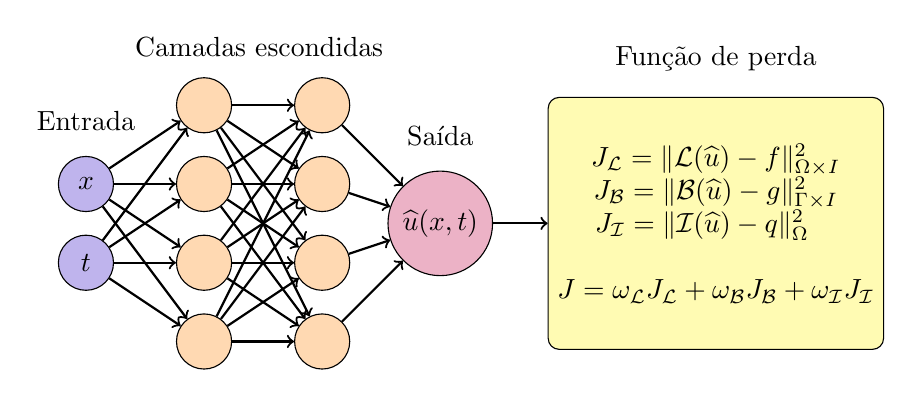
\begin{tikzpicture}[
    neuron/.style={circle, draw, minimum size=0.7cm},
    input/.style={neuron, fill=blue!30},
    hidden/.style={neuron, fill=orange!30},
    output/.style={neuron, fill=purple!30},
    physnode/.style={rectangle, draw, rounded corners, fill=orange!30, minimum width=1.5cm, minimum height=1.8cm},
    lossnode/.style={rectangle, draw, rounded corners, fill=yellow!30, minimum width=2cm, minimum height=3.2cm, align=center},
    every edge/.style={draw, ->, thick}
]

\node[input] (I-1) at (0, 2) {$x$};
\node[input] (I-2) at (0, 1) {$t$};

\node[hidden] (H1-1) at (1.5, 3) {};
\node[hidden] (H1-2) at (1.5, 2) {};
\node[hidden] (H1-3) at (1.5, 1) {};
\node[hidden] (H1-4) at (1.5, 0) {};

\node[hidden] (H2-1) at (3, 3) {};
\node[hidden] (H2-2) at (3, 2) {};
\node[hidden] (H2-3) at (3, 1) {};
\node[hidden] (H2-4) at (3, 0) {};

\node[output] (O-1) at (4.5, 1.5) {$\widehat{u}(x,t)$};

% Connections
\foreach \i in {1,2}
    \foreach \j in {1,...,4}
        \path (I-\i) edge (H1-\j);

\foreach \i in {1,...,4}
    \foreach \j in {1,...,4}
        \path (H1-\i) edge (H2-\j);

\foreach \j in {1,...,4}
    \path (H2-\j) edge (O-1);

\node[lossnode] (TotalLoss) at (8, 1.5) {
$J_{\mathcal{L}} = \lVert \mathcal{L}(\widehat{u}) - f \rVert^{2}_{\Omega \times I}$
\\
$J_{\mathcal{B}} = \lVert \mathcal{B}(\widehat{u}) - g \rVert^{2}_{\Gamma \times I}$
\\
$J_{\mathcal{I}} = \lVert \mathcal{I}(\widehat{u}) - q \rVert^{2}_{\Omega} \quad$
\\
\\
$J = \omega_{\mathcal{L}} J_{\mathcal{L}} + \omega_{\mathcal{B}} J_{\mathcal{B}} + \omega_{\mathcal{I}} J_{\mathcal{I}}$
};

\path (O-1) edge (TotalLoss);

% Labels
\node[above=0.2cm] at (I-1.north) {Entrada};
\node[above=0.2cm] at (2.2, 3.3) {Camadas escondidas};
\node[above=0.2cm] at (O-1.north) {Saída};
\node[above=0.2cm] at (TotalLoss.north) {Função de perda};

\end{tikzpicture}
\caption{Representação gráfica das PINNs. Fonte: elaborada pelos autores.}
\label{fig:pinn-representacao-grafica}
\end{figure}

A formulação acima vale tanto para problemas diretos, quanto para problemas 
inversos

\section{Modelos Compartimentais}

Baseados neste trabalho seminal,foram propostos outros modelos com mais mais 
compartimentos como o \textit{SEIRD} \cite{giles:77-sird} que inclui um 
compartimento para individuos que foram expostos a doença, mas 
ainda não manifestaram sintomas. 
Outro exemplo é o \textit{SIRV} \cite{schlickeiser-kroger:21-sirv} 
que inclui um compartimento para vacinados.

Em \cite{kendall:2023-modelos-epd-estocasticos}, é introduzido um modelo estocástico
baseado no trabalho já citado.

$R_0$ número básico

\begin{equation}
    R_0 = \frac{\beta}{\gamma}
\end{equation}

Apresentado no trabalho seminal de \cite{kermack-mcKendrick:1927}, o modelo 
\textit{SIR} é definido pelo conjunto de equações \ref{eq:SIR-1}, \ref{eq:SIR-2}
e \ref{eq:SIR-3}.

\begin{eqnarray}\label{eq:sir}
   \frac{dS(t)}{dt} &=& -\beta S(t) I(t),  \quad t > t_0, \label{eq:SIR-1}\\
   \frac{dI(t)}{dt} &=& \beta S(t) I(t) - \gamma I(t), \quad t > t_0, \label{eq:SIR-2}\\
   \frac{dR(t)}{dt} &=& \gamma I(t),  \quad t > t_0, \label{eq:SIR-3} \\
   S(t) + I(t) + R(t) &=& N,  \quad t > t_0, \label{eq:SIR-4}
\end{eqnarray}

O modelo pode ser entendido com um grafo\dots A figura \ref{fig:sir-grafo}
ilustra o modelo \textit{SIR}.

\begin{figure}
\centering
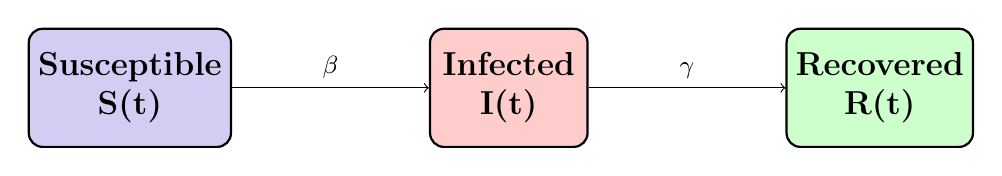
\begin{tikzpicture}[
    node distance=2.5cm,
    box/.style={rectangle, minimum width=2cm, minimum height=1.5cm, 
                draw=black, thick, align=center, rounded corners=5pt,
                font=\large\bfseries},
    arrow/.style={-Stealth, thick, line width=1.2pt},
    label/.style={midway, sloped, font=\small}
]

    % Define nodes
    \node[box, fill=blue!20] (S) {Susceptible \\ S(t)};
    \node[box, fill=red!20, right=of S] (I) {Infected \\ I(t)};
    \node[box, fill=green!20, right=of I] (R) {Recovered \\ R(t)};

    % Transitions
    \draw (S) edge[->] node[label,above] {$\beta$} (I);
    \draw (I) edge[->] node[label,above] {$\gamma$} (R);

\end{tikzpicture}
\caption{Grafo para o \textit{SIR}. Fonte: elaborada pelos autores.}
\label{fig:sir-grafo}
\end{figure}



\section{Problemas Inversos}

Problemas inversos são mal-postos\dots

Identificabilidade de um modelo\dots

\section{Aplicação de PINNs com Modelos Compartimentais}

\cite{}

Modelos de ordem facionária \cite{li-etal:25-ordem-fracionaria}

Sir reação-difusão \cite{bertaglia-etal:22-sir-reacao-difusao}

Um exemplo utilizando redes neurais recorrentes pode ser encontrado em \cite{rodriguez-etal:2022-einns}

No artigo original, são utilizados \textit{Multi-layer Perceptrons} (MLPs)
como arquitetura das redes, mas há propostas com utilizando outras arquiteturas.
Uma proposta utilizando redes neurais convolucionais pode ser encontrada em 
\cite{shi-etal:24-convnet}. Uma proposta utilizando PINNs combinado com 
métodos Bayesianos pode ser encontrada em \cite{yang:21-bpinns}, esta 
abordagem é particulamente interessante para problemas inversos, ao transformar
a estimativa dos parâmetros numa distribuição, no lugar de um valor fixo.

% ==============================================================================
% TCC - Nome do Aluno
% Capítulo 3 - Proposta do Trabalho
% ==============================================================================
\chapter{Proposta do Trabalho}
\label{sec-proposta}

Nesta seção é apresentada a proposta para a estimativa dos parâmetros do 
modelo compartimental e os testes para averiguar a efetividade do método.

\section{Estimativa de parâmetros}

Os modelos compartimentais possuem parâmetros de transmissão e mortalidade
fixos, considerando que estes modelos foram pensados apenas para dar 
uma projeção de como uma epidemia evoluirá. Entretanto, medidas de afastamento
social são capazes de alterar o parâmetro de transmissão ao longo do tempo.
Utilizando \cite{long-etal:21-L2} como inspiração, é proposto obter o parâmetro
$\beta$ como uma função em função do tempo. A rede neural deverá se ajustar 
a um $\beta(t)$. A taxa de mortalidade de uma doença permanece constante
caso não haja um plano de vacinação, logo não há a necessidade de estimá-lo. 

\begin{eqnarray}
   \frac{dS(t)}{dt} &=& -\beta(t) S(t) I(t),  \quad t > t_0, \label{eq:SIR-beta-t-1}\\
   \frac{dI(t)}{dt} &=& \beta(t) S(t) I(t) - \gamma I(t), \quad t > t_0, \label{eq:SIR-beta-t-2}\\
   \frac{dR(t)}{dt} &=& \gamma I(t),  \quad t > t_0, \label{eq:SIR-beta-t-3}
\end{eqnarray}

\section{Testes com Dados Sintéticos}

Para averiguar se o método proposto funcionará bem com dados reais,
será feito primeiramente um teste com dados sintéticos obtidos apatir da solução
do modelo compartimental utilizando o método de Runge-Kutta de 4º ordem
implementado na biblioteca \textit{SciPy} \cite{scipy}.

\begin{equation}
    \beta(t) = \sin(t / 12)  + \beta_{min}
\end{equation}

\section{Testes com Dados Sintéticos Ruidosos}

Segundo \cite{raissi-etal:19}, PINNs são resilientes a dados ruidosos. Para
testar se PINNs são capazes de ajustar a 
adicionar ruído gaussiano aos dados sintéticos. A equação \ref{eq:ruido-gaussiano}
descreve este processo.

\begin{eqnarray}\label{eq:ruido-gaussiano}
    Z_t \sim \mathcal{N}(0, \sigma) \\
    \mathcal{N}_t = \mathcal{C}_t + Z_t  
\end{eqnarray}

\section{Testes com Base de Dados Reais}

\subsection{Bases de dados do DataSUS}

\subsection{Tratamento dos Dados}
Janela móvel de 7 dias como em \cite{han-etal:24-prim-artigo-alemanha},
\cite{long-etal:21-L2} e \cite{shamsara-etal:25-omicron} para suavizar o ruído

Pesos ajustáveis entre a loss física e a loss dos dados como em
\cite{han-etal:24-prim-artigo-alemanha}, \cite{long-etal:21-L2} e 
\cite{shamsara-etal:25-omicron}

Segundo \cite{bonfanti-etal:24-generalizacao-pinns}, PINNs não generalizam bem
fora do domínio de treinamento. PINNs podem estimar os parâmetros para fora
do domínio de treinamento como em \cite{millevoi-etal:24-split-join-pinns}.

Assim como em \cite{ghosh-etal:23-subnotificacao}, fazer testes com lacunas
nos dados para testar a resiliência do método.

\subsection{Arquitetura da Rede}

Baseando-se em \cite{shaier-etal:22-dinns}, o número de camadas escolhido foi...

Como em \cite{millevoi-etal:24-split-join-pinns}, aplicar uma 
\textit{hard-constraint} na rede neural ao utilizar nos nós de saída
uma função de ativação que retorna apenas valores positivos.

\subsection{Correlação com a Temperatura}
% ==============================================================================
% TCC - Nome do Aluno
% Capítulo 3 - Avaliação do Trabalho
% ==============================================================================
\chapter{Avaliação do Trabalho}
\label{sec-avaliacao}

\section{Testes com Dados Sintéticos}

A figura \ref{fig:compartimentos-sir-semruido} mostra o valor de 
beta ao longo do tempo.

\begin{figure}[htpb]
\centering
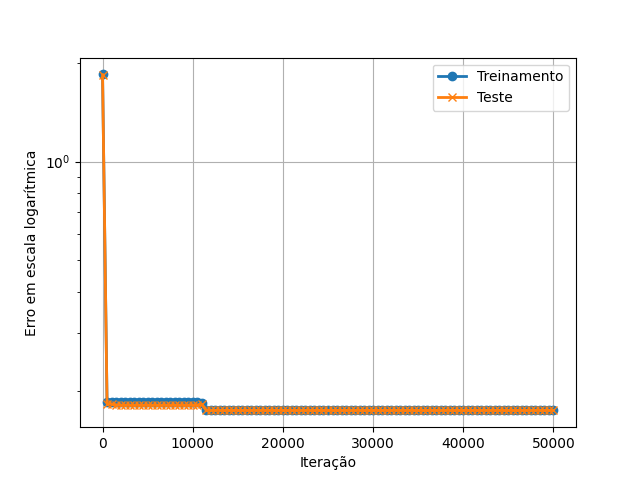
\includegraphics[width=0.6\textwidth]{figuras/loss-sir-nonoise.png}
\caption{Na primeira. Fonte: elaborada pelos autores.}
\label{fig:loss-sir-semruido}
\end{figure}


A figura \ref{fig:compartimentos-sir-semruido} mostra o valor de 
beta ao longo do tempo.

\begin{figure}[htpb]
\centering
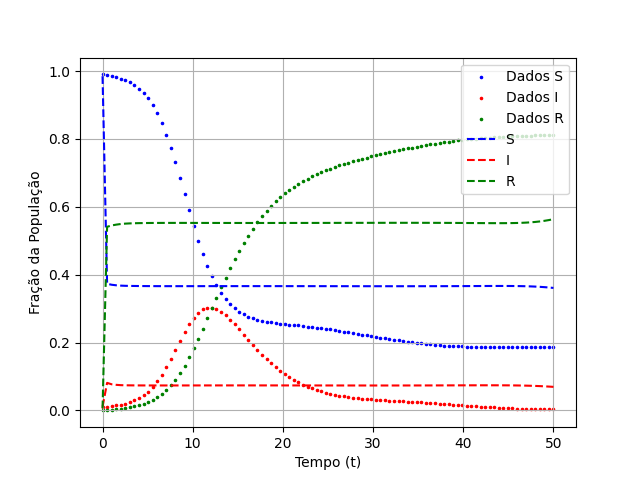
\includegraphics[width=0.6\textwidth]{figuras/predicted-compartments-sir-nonoise.png}
\caption{Na primeira. Fonte: elaborada pelos autores.}
\label{fig:compartimentos-sir-semruido}
\end{figure}

A figura \ref{fig:beta-sir-semruido} mostra o valor de beta ao longo do tempo.

\begin{figure}[htpb]
\centering
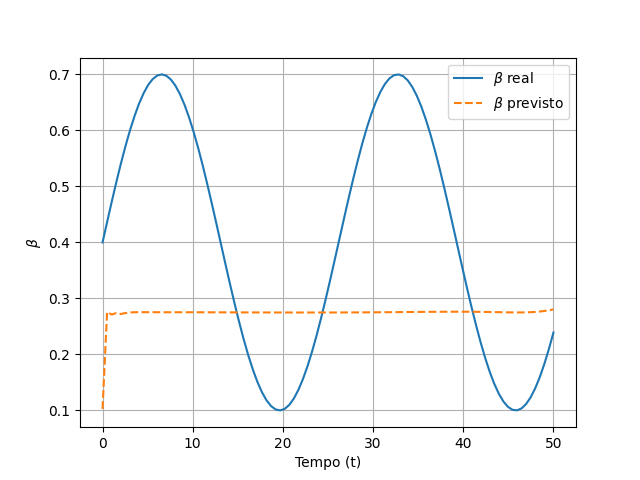
\includegraphics[width=0.6\textwidth]{figuras/predicted-beta-sir-nonoise.png}
\caption{Na primeira. Fonte: elaborada pelos autores.}
\label{fig:beta-sir-semruido}
\end{figure}


A tabela \ref{tab:metricas-dados-sinteticos} mostra os valores para 

\begin{table}[htpb]
\centering
\caption{Valores das métricas de erro (\textit{MSE}, norma $\mathcal{L}_2$ e norma $\mathcal{L}_\infty$) para as soluções aproximadas pela rede neural, em comparação com as soluções analíticas.}
\begin{tabular}{|c|c|c|c|}
\hline 
\hline 
\multirow{2}{*}{} & \multicolumn{3}{c|} {Métricas} \\ \cline{2-4} 
Compartimento & MSE & $\mathcal{L}_2$ & $\mathcal{L}_\infty$ \\ \hline
$S$ & $8{,}628 \times 10^{-6}$ & $2{,}444 \times 10^{-3}$ & $1{,}182 \times 10^{-2}$\\ \hline
$I$ & $1{,}005 \times 10^{-6}$ & $1{,}252 \times 10^{-2}$ & $4{,}81 \times 10^{-3}$\\ \hline
$R$ & $1{,}997 \times 10^{-6}$ & $4{,}913 \times 10^{-3}$ & $8{,}635 \times 10^{-3}$ \\ \hline
\hline
\end{tabular}
\label{tab:metricas-dados-sinteticos}
\end{table}


\section{Testes com Dados Ruidosos}

A figura \ref{fig:compartimentos-sir-semruido} mostra o valor de 
beta ao longo do tempo.

\begin{figure}[htpb]
\centering
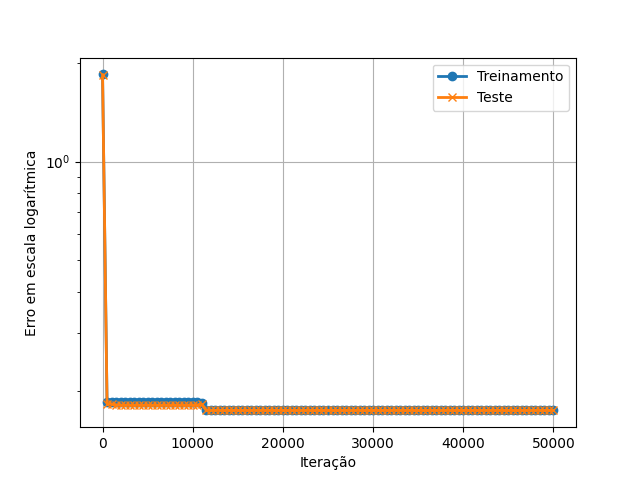
\includegraphics[width=0.6\textwidth]{figuras/loss-sir-nonoise.png}
\caption{Na primeira. Fonte: elaborada pelos autores.}
\label{fig:loss-sir-ruidoso}
\end{figure}


A figura \ref{fig:compartimentos-sir-ruidoso} mostra o valor de 
beta ao longo do tempo.

\begin{figure}[htpb]
\centering
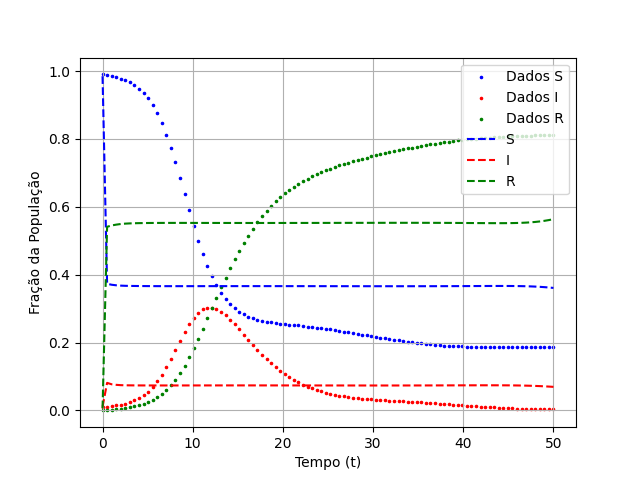
\includegraphics[width=0.6\textwidth]{figuras/predicted-compartments-sir-nonoise.png}
\caption{Na primeira. Fonte: elaborada pelos autores.}
\label{fig:compartimentos-sir-ruidoso}
\end{figure}

A figura \ref{fig:beta-sir-ruidoso} mostra o valor de beta ao longo do tempo.

\begin{figure}[htpb]
\centering
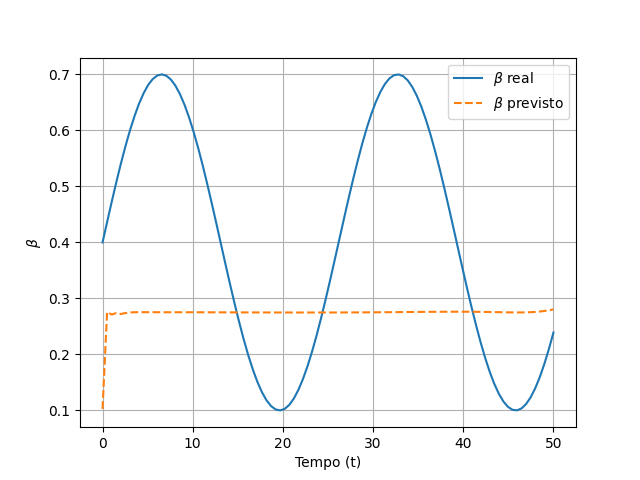
\includegraphics[width=0.6\textwidth]{figuras/predicted-beta-sir-nonoise.png}
\caption{Na primeira. Fonte: elaborada pelos autores.}
\label{fig:beta-sir-ruidoso}
\end{figure}


A tabela \ref{tab:metricas-dados-sinteticos-ruidosos} mostra os valores para 

\begin{table}[htpb]
\centering
\caption{Valores das métricas de erro (\textit{MSE}, norma $\mathcal{L}_2$ e norma $\mathcal{L}_\infty$) para as soluções aproximadas pela rede neural, em comparação com as soluções analíticas.}
\begin{tabular}{|c|c|c|c|}
\hline 
\hline 
\multirow{2}{*}{} & \multicolumn{3}{c|} {Métricas} \\ \cline{2-4} 
Compartimento & MSE & $\mathcal{L}_2$ & $\mathcal{L}_\infty$ \\ \hline
velocidade $u$ & $8{,}628 \times 10^{-6}$ & $2{,}444 \times 10^{-3}$ & $1{,}182 \times 10^{-2}$\\ \hline
velocidade $v$ & $1{,}005 \times 10^{-6}$ & $1{,}252 \times 10^{-2}$ & $4{,}81 \times 10^{-3}$\\ \hline
pressão $p$ & $1{,}997 \times 10^{-6}$ & $4{,}913 \times 10^{-3}$ & $8{,}635 \times 10^{-3}$ \\ \hline
\hline
\end{tabular}
\label{tab:metricas-dados-sinteticos-ruidosos}
\end{table}

\section{Testes com Base de Dados Reais}
% ==============================================================================
% TCC - Nome do Aluno
% Capítulo 3 - Considerações Finais
% ==============================================================================
\chapter{Considerações Finais}
\label{sec-conclusoes}

Aplicar PINNs Bayesianas \cite{yang:21-bpinns} para estimar o desvio 
padrão do $\beta(t)$.




%%% Páginas finais do documento: bibliografia e anexos. %%%

% Finaliza a parte no bookmark do PDF para que se inicie o bookmark na raiz e adiciona espaço de parte no sumário.
\phantompart

% Marca o início dos elementos pós-textuais.
\postextual

% Referências bibliográficas
\bibliography{bibliografia}


% Apêndices.
\begin{apendicesenv}

% Imprime uma página indicando o início dos apêndices.
\partapendices

% (*) Incluir como apêndice a documentação técnica produzida durante o TCC (especificação de requisitos,
% projeto arquitetural, etc.). Utilizar o exemplo \includepdf caso o documento seja produzido em outro
% editor de texto (Microsoft Word, LibreOffice Writer) e transformado em PDF. Utilizar o exemplo \include
% caso os documentos tenham sido também escritos em LaTeX.
% \includepdf[pages={1-}]{apendices/apendice01-requisitos.pdf}
% \includepdf[pages={1-}]{apendices/apendice02-projeto.pdf}
% \include{ap1-requisitos}
% \include{ap2-projeto}
\end{apendicesenv}


% Índice remissivo.
\phantompart
\printindex

% Fim do documento.
\end{document}
